% !TEX root = main.tex
\section{Head-aware Conceptualization (Online Answering)}
\label{sec:conceptualization}
In this section, we give our solution to compute $P(c|e_i)$, the probability that $c$ is a concept of entity $e_i$ using \ac{Probase}, a web-scale taxonomy.
As we have claimed, head-aware conceptualization is a distinguished feature of our problem.
We first motivate this problem. Then give our solution.
%\nop{
%We first briefly introduce Probase and give a direct solution.
%However, the direct conceptualization solution ignores the unique setting of relationship explanation.
%We will analyze the problems caused by our problem setting then give an improved version.
%}

%\nop{
%\subsection{Problem Statement}
%
%Given an entity, our target in this section is to find its rich probabilistic representation by concepts.
%The \term{type} information from knowledge database such as Yago, DBpedia can be utilized to represent concepts as an option.
%Nevertheless, we envision that applying probabilistic representation such as using concepts in \ac{Probase} will fit our problem better.
%
%Probase exploit Hearst patterns to extract isA relations from 1.68 billion web pages .
%For example, it extracts evidence for the claim \at{IBM \isa company, Nokia \isa company} from sentence \at{...\ac{companies} such as \ac{IBM, Nokia}...}
%The core version of Probase contains 3,024,814 unique concepts, 6,768,623 unique instances, and 29,625,920 isA relations.
%
%Given an entity $e$, from Probase, we can acquire its concepts' set $C(e)$.
%For each $c_i \in C$, the frequency $n(c_i,e)$ can be accordingly derived, which means how many times the $e$ isA $c$ can be observed from the corpus.
%The frequency information allows us to estimate  $P(c|e)$ by
%$$P(c|e)=\frac{n(c,e)}{\sum_{c_i\in C(e)}n(c_i, e)}$$
%}


\subsection{Head-aware Conceptualization}
We further argue that the relationship between entities are determined by the head concepts, as illustrated in Example~\ref{exa:hc}.
%For example, the \at{FoundedBy} relationship between \at{Apple Inc.} and \at{Steve Jobs} are determined by the head concepts they possessed (e.g.\ \term{company} and \term{entrepreneur}, regardless of the modifiers such as \term{technology} in the concept \term{technology company}.)
Hence, the attribute should be generated by the head concept pairs instead of the modified concept pairs.
This motivates us to refine the optimization objective by summing over on the head concept pairs.
Let $\bar{C}_1$ and $\bar{C}_2$ be the head concepts in  $C_1$ and $C_2$, respectively.
Our problem is refined as to be:
\begin{equation}
\label{eq:target_head}
\small
\argmax_a \sum_{c_i\in \bar{C}_1 , c_j \in \bar{C}_2 } P(a|\langle c_{i},c_{j} \rangle \times P(\langle c_{i},c_{j}\rangle|\langle e_{1},e_{2}\rangle)
\end{equation}

By restricting the concept to the head concept, we can further reduce the computation cost.
The number of head concept pairs is obviously significantly smaller than that of the concept pair and that of entity pairs.
Because most concepts are tail concepts with long modifiers.
\nop{Our statistics show that there are only 33197 head concepts, which is significantly less that 2 million original concepts in Probase.
By focusing on head concept, we can effectively find the relationships without handling the huge number of long-tailed concepts and their entities.
}
\paragraph*{Probase}
We use Probase to do conceptualization of entities. 
%Probase exploit Hearst patterns to extract isA relations from 1.68 billion web pages. For example, it extracts \at{IBM} isA \at{company}, \at{Nokia} isA \at{company} relationships from sentence \at{...\ac{companies} such as \ac{IBM, Nokia}...}
Probase contains isA relations between entities and concepts. It contains 3 millions of concepts, 6 millions of instances, and almost 30 millions of isA relations.
Given an entity $e$, let its concept set in Probase be $C(e)$.
Each $e$ isA $c$ relations is associated with a frequency, denoted by $n(e, c)$.
Thus we can estimate  $P(c|e)$ by
$P(c|e)=\frac{n(c,e)}{\sum_{c_i\in C(e)}n(e, c_i)}$.

\paragraph*{Finding Head Concepts}
We use the following procedure to get head concept for an entity $e$.
We first retrieve all concepts of $e$ in Probase. Let the set of these concepts be $C(e)$.
Then, we reduce $C(e)$ to $\bar{C}(e)$ so that each concept in $\bar{C}(e)$ contains all {\bf head} of each concept in $C(e)$.
We identify the head concept by syntax-based patterns~\cite{ponzetto2007deriving} for noun phrases.
We denote each head concept as $h$ and a concept with modifiers as ${l}$.
We use $H(e)$ to denote the set of head concepts of $e$.
Our problem is reduced to the recalculation of the probability $P({h}|e)$.


\subsection{Conceptualization into Head Concepts}
One problem in the estimation of $p(h|e)$ is that we are likely to underestimate $p(h|e)$ because in general there is no sufficiently direct isA relationships from entity $e$ to the head concept $h$.
We illustrate this in Example~\ref{exa:conc}.

{\footnotesize
%For our task, we only need relatively general concepts(a.k.a. head concepts).
\begin{example}[Underestimation]
\label{exa:conc}
Consider the entity \ac{Thomas Watson}, by whom \ac{IBM} was founded. Its concepts in Probase include \ac{\{success leader,modern day entrepreneur,... \}}. The isA link from \at{Thomas Watson} to \at{entrepreneur} is however missing since we always refer to \at{Thomas Watson} as a modern day entrepreneur. The direct computation yields $P(\ac{entrepreneur}|\at{\text{Thomas Watson}})=0$, which is obviously an underestimation.
\end{example}
}


%\yh{in experiments, we should compare the baseline that directly use concepts instead of head concepts.}
%\nop{
%\begin{example}[Head concepts VS Original concepts]
%\label{exa:HvsO}
%Take \term{famous painting} as example. Its original concepts are \term{image, treasure}, which are reasonable but not plausible, since their occurrence are 2 and 1 respectively. However, the most plausible concept \term{painting} is not among the concepts.
%\end{example}
%}
%\yh{Rewrite the objective function when we only consider the head concepts}
%
%\nop{
%\paragraph{The main steps of conceptualization}
%Given an entity $e$ from $Probase$, where we can get its concepts.
%First we do head modifier detection based on syntax[], since the concepts in Probase all follows English grammar, this approach already produces a good result.
%Next, we recalculate the probability of $P({c_h}|e)$ by aggregating the contribution from $c_l$.
%The essentiality of doing so is illustrated in Example~\ref{exa:recalc}.
%Finally, we provide a method to take the original isA relation from Probase into consideration.
%
%\begin{example}[Essentiality of Aggregation]
%\label{exa:recalc}
%\term{Steve Jobs} The concept \term{well-known name} has four occurrences however \term{name} has only 2. There are other modifiers for the same head, so that the typicality of the head will be largely underestimated.
%\end{example}
%}

\subsubsection{Baseline}
The underestimation is caused by the ignorance of mentions of a entity as an instance of modified concepts. As shown in Example~\ref{exa:clc}, we should count the number that $e$ isA ${l}$ when we count the $e$ isA ${h}$ for any $l$ that is a modified concept of $h$.
Hence, the most straight forward approach is rectifying the $n(e, h)$ by the additional count
of all $n(e, l)$ such that $h(l)=h$, where $h()$ is a function that generate the head concept of a long concept. The rectification of count and corresponding rectified estimation are shown in Eq~\ref{eq:rec}. 
%According to the rectified count, we have a rectified estimation on $P(h|e)$, as shown in Eq~\ref{eq:recp}.
\begin{equation}
\small
\hat{n}(h, e)={n}(h, e)+\sum_{ h(l)=h} n(l,e), \hat{P}(h|e)=\frac{\hat{n}(h, e)}{\sum_{{h'}}{\hat{n}({h'}}, e)}
\label{eq:rec}
\end{equation}



{\footnotesize
\begin{example}[Rectification by Modified Concepts]
\label{exa:clc}
As illustrated in Figure~\ref{fig:pgge}, in Probase, \at{Bill Gates} isA  \at{Leader} and \at{Bill Gates} isA \at{Business Leader} are observed respectively 9 times and 17 times from corpus. Since \at{Business Leader} is always a \at{Leader},  logically, \at{Bill Gates} isA \at{Leader} was observed 26 times instead of 9 times.
\end{example}
}

\subsubsection{Improvement by Concepts with Different Heads}
Except the modified concepts of a head, there are some other concepts that has different heads but  are semantically subclasses of the head concept. These subconcepts should be taken into account to estimate the ${P}(h|e)$.  We illustrate the rationality in Example~\ref{exa:isagood}.

{\footnotesize
\begin{example}[Concepts with Different Heads]
\label{exa:isagood}
For example in Figure~\ref{fig:pgge}, \at{Bill Gates} has isA links to \at{successful entrepreneur} and \at{Industry Leader}. These two concepts has isA links to \at{business leader} and \at{Industry Leader}, respectively.  which is reasonable. Although these two concepts are not the modified concepts of \at{Leader}, their mentions as a concept of \at{Bill Gates}  should be considered when estimating $P(\at{Leader}|\at{Bill Gates})$.
\end{example}
}

%\vspace{-1mm}
\begin{figure}[!tb]
\vspace{-8mm}
\label{fig:pgge}
\centering
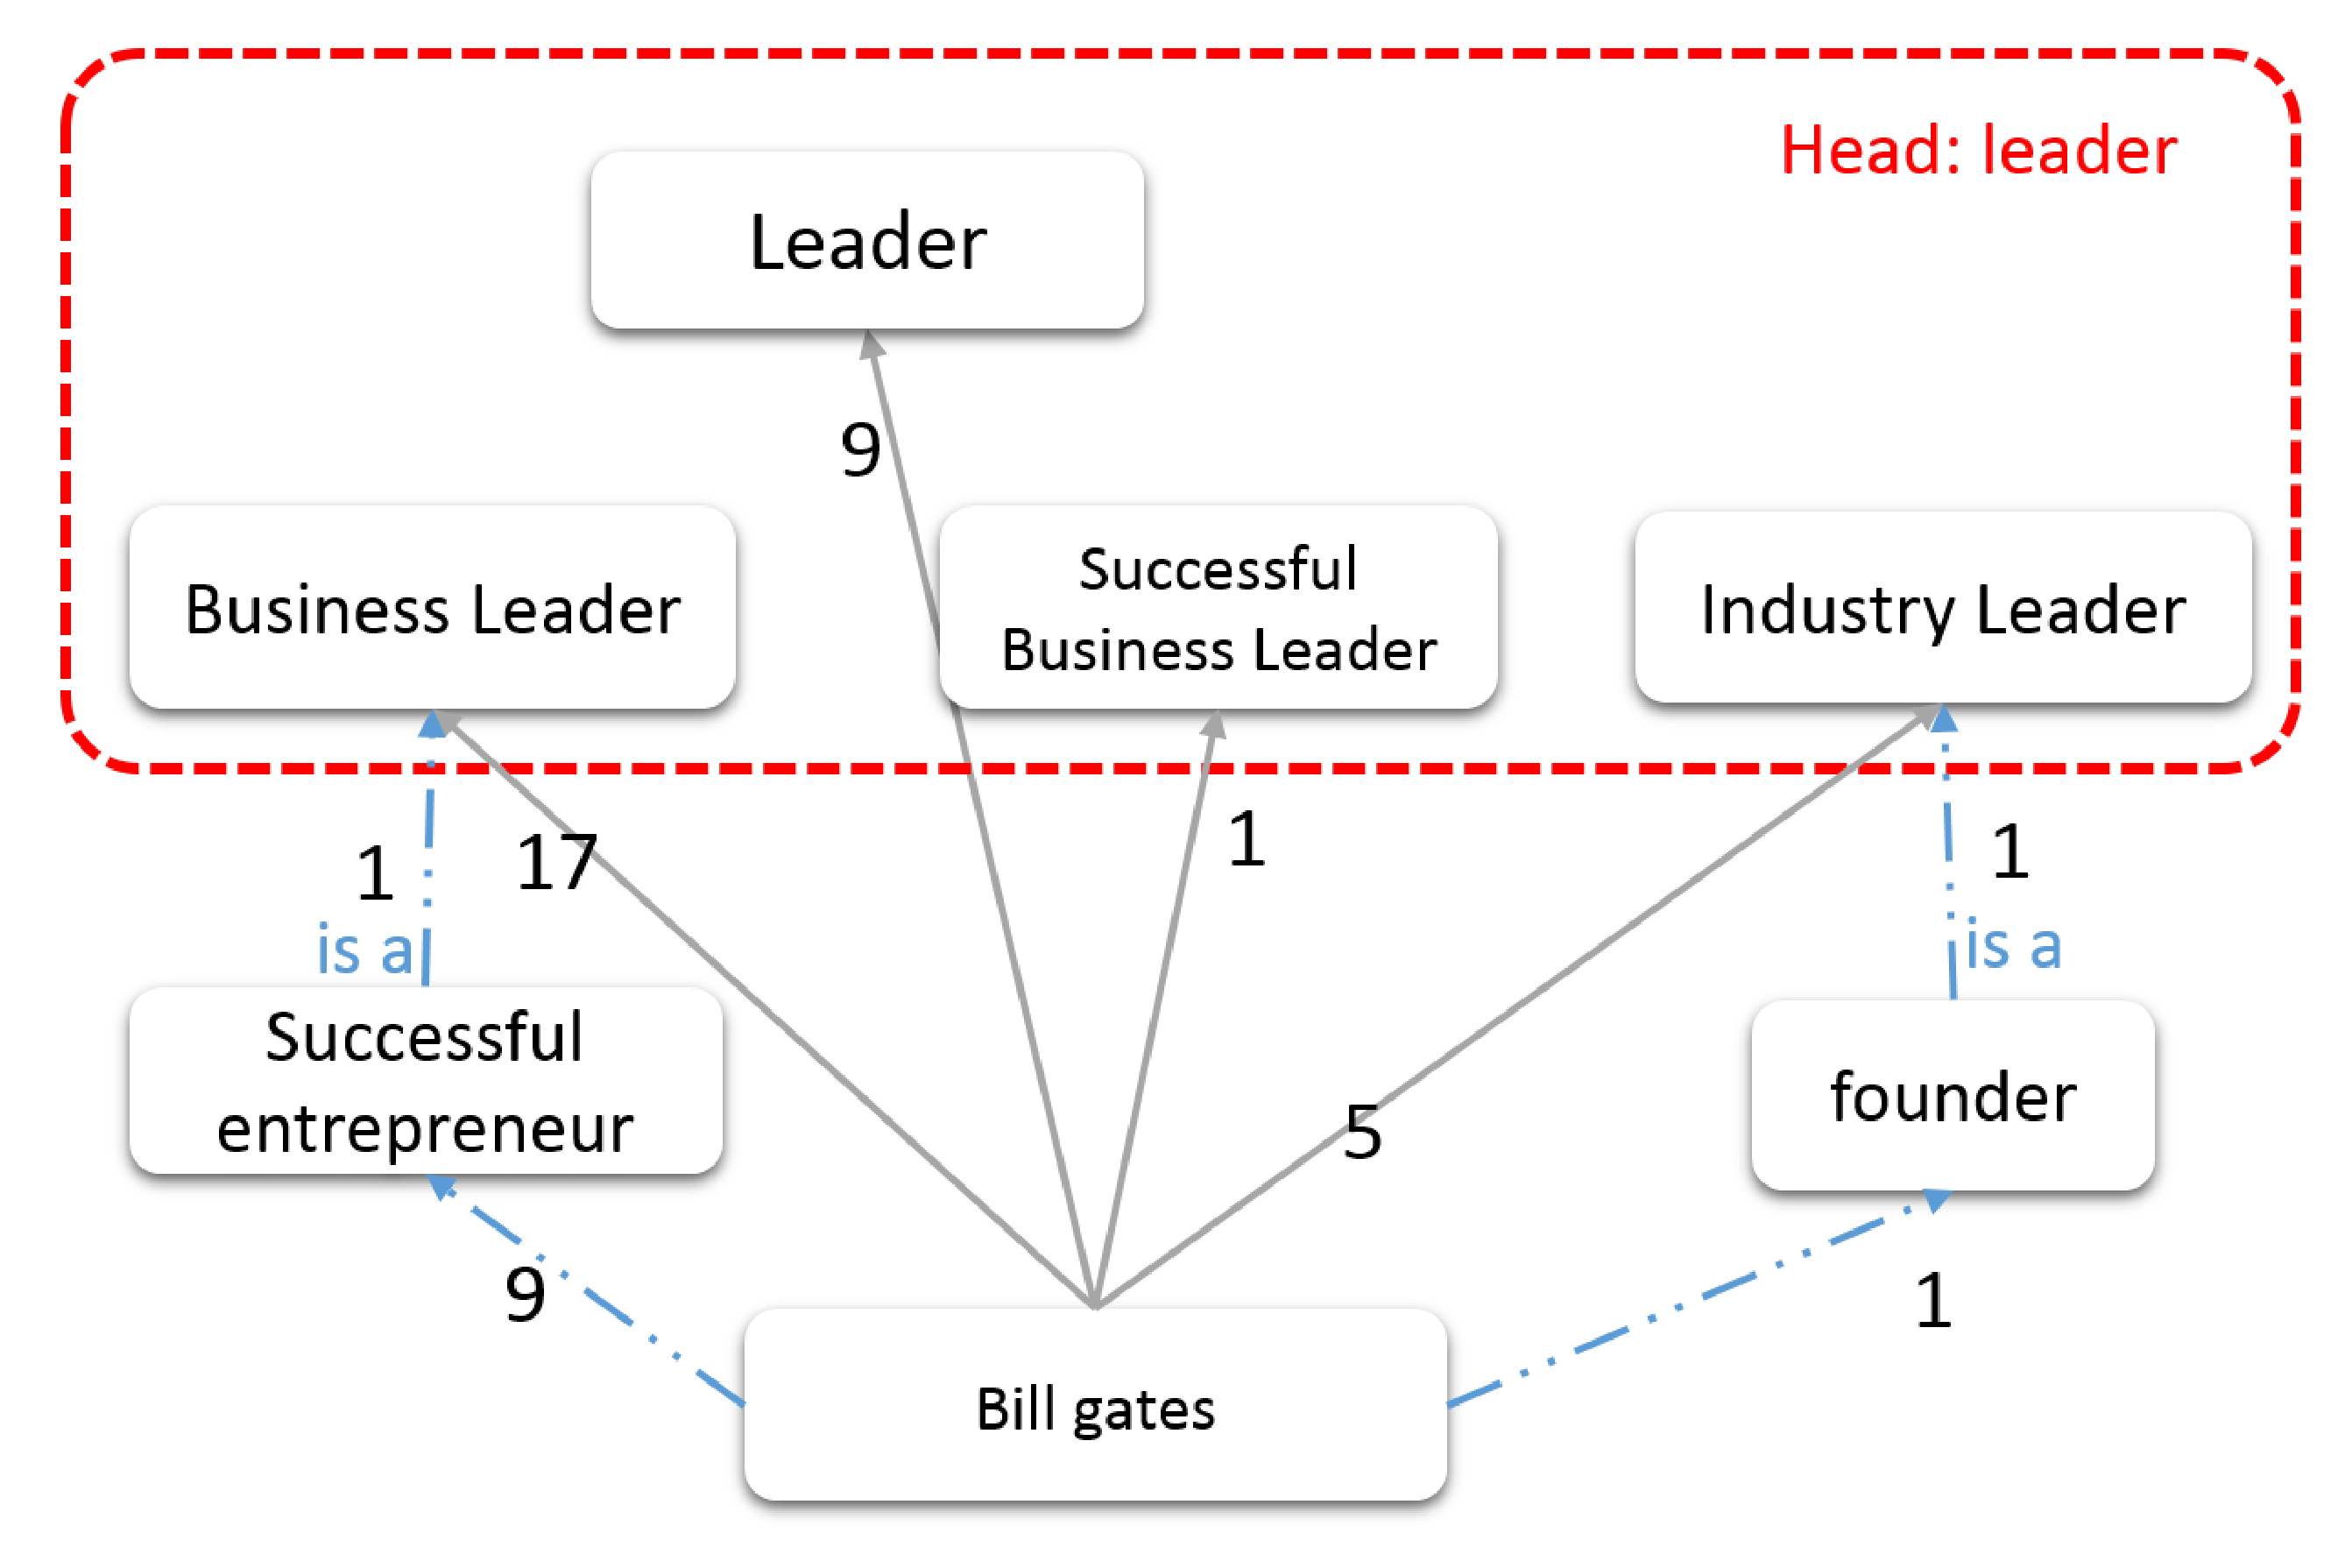
\epsfig{file=resources/bill_gates_isa.eps,width=\columnwidth, height=0.4\columnwidth}%5.5in
%考虑 transitivity: e \isa $c_l$ \isa $c_h$,  e \isa $c_l$* transitivity_coeff(cl->ch) = e \isa ch
\vspace{-4mm}
\caption{Calculation of $P({c}|\term{Bill Gates})$ }
\vspace{-3mm}
\end{figure}

%%%%%%%%%%%%%%%%%%%%%%%%%%%%%%%%%%
%\nop{
%In both case B.1 and B.2, the weight of the edge $c_{l}$ \isa ${c_h}$ is underestimated. We argue that when calculating the typicality $P({c_h}|e)$, the counts of the long concept contributing to its head concept should be re-estimated as follows.
%
%Notice that the boundary between case B.1 and case B.2 are not strict, there are such edges that have low observation in Example~\ref{exa:HvsO}. So that if we consider them as a whole, we can derive:
%\begin{equation} P({c_h}|c_{l})=\lambda P_{head}({c_h}|c_{l})+(1-\lambda)P_{probase}({c_h}|c_{l}) \label{eq:pcgclong}\end{equation}
%where $\lambda$ is a parameter \xch{principle: related to plausibility, number of occurrence, varies for different $c_{l}$ should it be derived from learning ?} since we assume $P_{head}({c_h}|c_{l})$ to be 1, Eq.~\ref{eq:pcgclong} is simplified to:
%$$P({c_h}|c_{l})=\lambda  +(1-\lambda)P_{probase}({c_h}|c_{l}) $$
%}
%%%%%%%%%%%%%%%%%%%%%%%%%%%%%%%%%%%%
Now we elaborate how to take into account the subconcepts with different heads. We first argue that we can not directly count its number of isA mentions like Eq~\ref{eq:rec}. Because its mentions should be contributed to its own head. For example, for \at{successful entrepreneur}, the number of \at{Bill Gates} isA \at{successful entrepreneur} should be attributed to \at{entrepreneur} instead of \at{Leader}.
Hence, we need a new framework.

Instead of direct lying rectifying the isA count, we rectify the conditional probability in Eq.~\ref{eq:recp} by counting additional probability contributed by subconcepts with different heads. Given an entity $e$ and one of its head concept $h$, let $C_h$ be the set of all $h$'s modified concepts and $h$ itself. Let $C^*_h$ be all concepts with different heads but having a isA link to one concept in $C_h$. We quantify how likely an entity $e$ reaches to any one concept in $C_h$ by a random walk procedure. In the random walk procedure, we use $P(c|e)=\frac{n(c,e)}{n(e)}$ as the random walk probability from $e$ to $c$. We can similarly define $P(c_1|c_2)$ when $c_2$ is a subconcept of $c_1$.  Thus, we need to aggregate all the random walk probability from $e$ to any concept in $C_h$.
Hence, our improved estimation of $P({c_h}|e)$ is as follows:
\begin{equation}
\small
\hat{P}({h}|e) = \gamma \hat{P}({h}|e)+ (1-\gamma) \sum_{c_i\in C^*_h}\sum_{ c_j\in C_h} P(c_j|c_i) P(c_i|e)
\label{eq:pgge}
\end{equation}
where we use $\gamma$ to tune relative importance of two parts and $1-\gamma$ part is the contribution from the subconcepts with different heads.


Note that we only consider two-steps of random walk due to the following reasons.
First, long-steps random walk tend to introduce too general or non-related concepts such as \term{issue, factor, element}, which are concepts for almost all the entities.
Second, random walk of long steps in general is costly since most real graphs are small-world.
%bill gates 的例子OK 么, 如果OK 我开始写example of calculation

%
%The process of calculation is illustrated in the example~\ref{exa:calc}
%
%\begin{example}[Calculating $P({c_h}|e)$]
%\label{exa:calc}
%As illustrated in Fig.~\ref{fig:pgge}, the process of calculating the typicality a concept is as follows, where \term{painting} is ${c_h}$ and \term{Mona Lisa} is $e$. Then $P(\term{painting}|\term{Mona Lisa})$ consists of 2 parts, the direct edge $P_{original}({c_h}|e)= 0.23$, and the second part
%$$\sum_{ c_{l}^*\in C_{l} } [ \lambda_{i}^*+(\alpha_{i}^*) P({c_h}|c_{l}^*) ] \times  P(c_{l}^*|e) $$
%$(\alpha_i^*+{c_h}^*=1)$
%Thus we get
%$$ P = 0.007\times \lambda_{i2}+0.05\times \lambda_{i1}+0.04\times(\lambda_{i3}+0.65\alpha_{i3}) $$
%For \term{piece}, it is the similar process. The relation here is only part of the whole graph.
%\end{example}

%\begin{tikzpicture}[->,>=stealth',shorten >=1pt,auto,node distance= 3 cm,
%  thick,main node/.style={circle,fill=blue!10,draw,font=\sffamily\bfseries,align = center}]
%
%  \node[main node] (4) {piece};
%  \node[main node] (2) [left of=4] {painting};
%
%  \node[main node] (5) [below of=2] {oil painting};
%  \node[main node] (6) [left of=5] {famous\\painting};
%  \node[main node] (7) [left of=6] {world's\\most famous\\painting};
%
%  \node[main node] (10) [right of=5] {art piece};
%  \node[main node] (11) [right of=10] {historical\\art piece};
%
%  \node[main node] (12) [below of=6] {Mona lisa};
%
%
%  \path[every node/.style={font=\sffamily\small}]
%
%    (5) edge  node [left] {$\lambda_{i3}$} (2)
%        edge [bend right] node [right] {\small{$ 0.65\alpha_{i3} $}} (2)
%        edge  [bend right] node[left]  {\small{$ 0.28\alpha_{i3} $}} (4)
%    (6) edge [bend left] node [right] {$\lambda_{i1}$} (2)
%    (7) edge [bend left] node [right] {$\lambda_{i2}$} (2)
%
%    (10) edge [bend right] node[right] {$\lambda_{i4}$} (4)
%    (11) edge node[right] {$\lambda_{i5}$} (4)
%    (12) edge [bend right]node[right] {0.01} (10)
%         edge [bend right]node[right] {0.007} (11)
%         edge node[right] {0.04} (5)
%         edge node[right] {0.05} (6)
%         edge node[right] {0.007} (7)
%         edge node[left] {0.23} (2)
%         edge [bend right]node[right] {0.04} (4);
%
%\end{tikzpicture}
